\documentclass[conference]{IEEEtran}

\usepackage{cite}
\usepackage{amsmath,amssymb,amsfonts}
\usepackage{algorithmic}
\usepackage{graphicx}
\usepackage{textcomp}
\usepackage{xcolor}
\usepackage{hyperref}
\def\BibTeX{{\rm B\kern-.05em{\sc i\kern-.025em b}\kern-.08em
    T\kern-.1667em\lower.7ex\hbox{E}\kern-.125emX}}

\hypersetup{
	colorlinks=true,
	linkcolor=black,
	filecolor=black,      
	urlcolor=black,
	citecolor=black
}
\begin{document}

\title{A Tree-Based Approach to Modeling Client Subscription Likelihood for Term Deposits}

\author{\IEEEauthorblockN{Gabriel Guillen}
\IEEEauthorblockA{\textit{dept. of Statistics \& Data Science} \\
\textit{University of Central Florida}\\
Orlando, United States of America \\
ga013701@ucf.edu}}


\maketitle
\renewcommand{\abstractname}{Summary}
\begin{abstract}
The primary aim of this study is a comparative performance analysis of three tree-based modeling techniques: a baseline \textbf{Decision Tree}, a \textbf{Bagging} ensemble, and a \textbf{Random Forest} classifier. The target variable is the binary subscription status (``yes'' or ``no'') of bank clients. By benchmarking these models, the study seeks to determine the superior predictive framework, with particular emphasis on navigating class imbalance through metrics of \textit{Recall}, \textit{F1-Score}, and overall generalization stability.\\
\end{abstract}

\section{\textbf{Introduction}}
\indent Tree-based models are frequently leveraged in financial modeling due to their inherent interpretability and robust generalization capabilities. Consequently, this study utilizes observations from a Portuguese banking institution's telemarketing campaign to perform a comparative performance analysis across three distinct configurations: a baseline \textbf{Decision Tree}, \textbf{Bagging} (Bootstrap Aggregating), and \textbf{Random Forest}.

The primary objective is to develop a predictive framework capable of classifying client propensity to subscribe to term deposits based on a multi-dimensional feature set. A critical constraint in this analysis is the significant class imbalance within the dataset, where approximately 88\% of observations belong to the negative class (``No''). In such an asymmetric distribution, a baseline Decision Tree is susceptible to majority class bias, often optimizing for global accuracy while failing to identify the minority class (``Yes'').

To mitigate this, ensemble models are employed to provide superior stability; by utilizing bootstrap sampling and feature randomness, these models reduce inherent variance to improve \textit{Recall} and \textit{F1-Score} for the minority class. This investigation focuses on the capacity of ensemble methods to effectively partition the feature space and capture nuanced subscriber signatures without overfitting to majority-class noise.

\subsection{\textbf{Dataset Structure}}
\indent The dataset \cite{moro2014} consists of 45,211 observations across 17 categorical and integer features. Given that tree-based models utilize recursive partitioning, the algorithms remain robust to mixed data types.\\
\indent Data auditing confirmed no null values; however, ``unknown'' labels within categorical features were preserved as valid attributes to maintain the integrity of the feature space and capture potential latent information. \\

\section{\textbf{Methods}}

\subsection{\textbf{Data Preparation}}

\subsubsection*{\textbf{Preprocessing}}
The data required minimal preprocessing, preserving the raw feature distribution for model training. The dataset was partitioned into a 90/10 training-to-test split using a randomized stratification approach to ensure representative class distributions across both subsets.\\ 
\indent The training set comprised 40,691 observations (35,930 ``No''; 4,761 ``Yes''), while the test set contained 4,520 observations (3,992 ``No''; 528 ``Yes''). Given the absence of null values and the native capacity of the R-based implementations to handle categorical factors, the models were trained on the original feature space. This preserved the structural integrity of the variables and maintained model interpretability without the need for manual dummy-variable transformation.

\subsection{\textbf{Tree-Based Models Used}}

\begin{enumerate}
	\item \textbf{Decision Tree}: This non-parametric baseline partitions the feature space into a hierarchy of axis-aligned rectangles by recursively maximizing information gain. While highly interpretable, a single tree is prone to high variance and "greedy" optimization, which in imbalanced financial datasets often leads to a majority-class bias that ignores the minority subscription class.
	\item \textbf{Bagging (Bootstrap Aggregating)}: Bagging reduces model variance by training multiple decision trees on different bootstrap samples of the original data and averaging their predictions. This ensemble approach stabilizes the decision boundary against the "noise" of the 88\% majority class, ensuring that the final classification is not overly sensitive to specific outliers in the training set.
	\item \textbf{Random Forest}: An extension of Bagging, Random Forest introduces feature decorrelation by selecting a random subset of predictors at each node split. This prevents a few dominant features from overshadowing more "nuanced" subscriber signatures, forcing the ensemble to explore a more diverse range of predictive patterns and significantly improving the F1-Score for the minority class.\\
\end{enumerate}

\newpage
\subsection{\textbf{Tuning and Selection}}
\subsubsection*{\textbf{Model Setup}}
To ensure a rigorous comparison, the experimental framework was initialized with specific hyperparameters and architectural constraints for each candidate model.

\begin{table}[ht]
	\centering
	\caption{Training Metadata and Model Configurations}
	\label{tab:model_configs}
	\begin{tabular}{lccc}
		\hline \hline
		\textbf{Configuration} & \textbf{Decision Tree} & \textbf{Bagging} & \textbf{Random Forest} \\
		\hline
		Target Column    & target        & target        & target        \\
		Model Type       & Decision Tree & Bagging       & Random Forest \\
		Number of Trees  & 1             & 25            & 100           \\
		OOB Error        & N/A           & 0.0991        & N/A           \\
		\hline \hline
	\end{tabular}
\end{table}


Table \ref{tab:model_configs} outlines the training metadata and structural differences between the baseline and ensemble methods. While the baseline Decision Tree provides a singular, high-variance path for classification, the Bagging and Random Forest configurations leverage 25 and 100 trees, respectively, to stabilize predictions.\\
\indent Notably, the Bagging model recorded an Out-of-Bag (OOB) error of approximately 0.0991, providing an early internal validation estimate of the model's generalization error without the need for a separate validation set.\\

\subsubsection*{\textbf{Pruning and Complexity}}
The Decision Tree was trained using default stopping criteria to establish a stable performance benchmark. 

\begin{table}[ht]
	\centering
	\caption{Decision Tree Complexity Table}
	\label{tab:cp_table}
	\begin{tabular}{ccccc}
		\hline \hline
		\textbf{CP} & \textbf{nsplit} & \textbf{rel error} & \textbf{xerror} & \textbf{xstd} \\
		\hline
		0.0372 & 0 & 1.0000 & 1.0000 & 0.0136 \\
		0.0256 & 3 & 0.8885 & 0.8901 & 0.0129 \\
		0.0162 & 4 & 0.8628 & 0.8675 & 0.0128 \\
		0.0102 & 5 & 0.8467 & 0.8519 & 0.0127 \\
		0.0100 & 7 & 0.8263 & 0.8502 & 0.0127 \\
		\hline \hline
	\end{tabular}
\end{table}

The relationship between the complexity parameter (CP) and the model's error rate is detailed in Table \ref{tab:cp_table}. As the number of splits ($nsplit$) increases, the cross-validation error ($xerror$) demonstrates a steady decline, eventually converging at $CP = 0.01$ with a minimum error of $0.8502$.\\
\indent This convergence ensures the baseline tree is sufficiently regularized, providing a robust foundation for comparison against the ensemble models.\\

\subsubsection*{\textbf{Feature Interpretability}}
Beyond predictive accuracy, a primary goal of this investigation is to isolate the specific drivers of client conversion. As a preliminary diagnostic, the Random Forest model is utilized to extract "Class-Specific Importance" metrics, offering an initial look at how individual features contribute to the classification of both "No" (non-subscribers) and "Yes" (subscribers).

\begin{table}[ht]
	\centering
	\caption{Random Forest Class-Specific Importance}
	\label{tab:rf_class_imp}
	\begin{tabular}{lccc}
		\hline \hline
		\textbf{Feature} & \textbf{Impact on 'No'} & \textbf{Impact on 'Yes'} & \textbf{MD-Gini} \\
		\hline
		duration  & 62.6994 & 129.2110 & 2304.3142 \\
		housing   & 21.3187 & 11.0848  & 148.3181  \\
		month     & 46.3405 & 11.4474  & 997.5681  \\
		job       & 18.5627 & -3.5030  & 556.8532  \\
		\hline \hline
	\end{tabular}
\end{table}

\newpage As a preliminary diagnostic, the \textbf{Random Forest} model was utilized to extract class-specific importance metrics, as shown in Table \ref{tab:rf_class_imp}. The variable \texttt{duration} (the length of the last contact) emerged as the most significant predictor for both classes, demonstrating an exceptionally high impact on the ``Yes'' class (129.21) and the highest Mean Decrease in Gini (MD-Gini).\\
\indent While these initial rankings provide a snapshot of the model's decision-making logic, a more exhaustive evaluation of feature interactions and stability across all  methods will be provided later in this report.

\section{\textbf{Results}}

Table \ref{tab:model_comparison} outlines a comparative analysis across the three model configurations, revealing a clear progression in predictive efficacy, particularly regarding the minority ``Yes'' class. While all models maintain a high overall accuracy ($\approx$ 91\%), this metric is primarily a reflection of the 88\% majority-class prevalence and does not fully capture the models' ability to identify subscribers.\\
\indent The most significant evolution is observed in the transition from the baseline to ensemble methods; the \textbf{Decision Tree} exhibits the lowest \textit{Recall} (0.4375), identifying fewer than half of actual subscribers and confirming its susceptibility to majority-class bias.
 
 \begin{table}[ht]
 	\centering
 	\caption{Comparison of Tree-based Models (Target: 'yes')}
 	\label{tab:model_comparison}
 	\begin{tabular}{lccc}
 		\hline \hline
 		\textbf{Metric} & \textbf{Decision Tree} & \textbf{Bagging} & \textbf{Random Forest} \\
 		\hline
 		Overall Accuracy & 0.9038 & 0.9024 & 0.9106 \\
 		Precision (Yes)  & 0.6260 & 0.5982 & 0.6455 \\
 		Recall (Yes)     & 0.4375 & 0.5019 & 0.5208 \\
 		F1-Score (Yes)   & 0.5151 & 0.5458 & 0.5765 \\
 		\hline
 		False Positives  & 297    & 263    & 253    \\
 		True Positives   & 231    & 265    & 275    \\
 		\hline \hline
 	\end{tabular}
 \end{table}
 
 In contrast, \textbf{Bagging} increases \textit{Recall} to 0.5019 by reducing model variance through bootstrap aggregation, though it experiences a slight ``Precision penalty'' (0.5982) due to more aggressive classification.\\
 \indent The \textbf{Random Forest} model achieves the peak performance across all minority-specific metrics, reaching a \textit{Recall} of 0.5208 and an \textit{F1-Score} of 0.5765. By simultaneously yielding the highest \textit{Precision} (0.6455) and the lowest count of \textit{False Positives} (253), the Random Forest demonstrates the most robust decision boundary for this asymmetric financial dataset, effectively isolating nuanced subscriber patterns that the baseline fails to capture.

\section{\textbf{Discussion}}

\subsection{Feature Importance}

As illustrated in Figure \ref{Tc_top_7_features}, while \texttt{duration} remains the primary feature across all three models, the relative importance of secondary features varies significantly. For instance, the \textbf{Decision Tree} relies heavily on \texttt{poutcome}, whereas \textbf{Bagging} assigns substantially higher relative importance to \texttt{age} and \texttt{month}.

\begin{figure}[htbp]
	\centerline{
\includegraphics[scale=0.45]{top_7_features_heatmap.png}}
	\caption{Top Features Models Agreed On}
	\label{Tc_top_7_features}
\end{figure}

Below these primary drivers, the models begin to stratify. While \texttt{month} and \texttt{poutcome} serve as a consistent secondary core, the ensemble methods exhibit a clear ``smoothing'' effect compared to the standalone Decision Tree. The \textbf{Decision Tree} (DT) column shows a sharp drop-off into lighter gradients for features such as \texttt{age}, \texttt{job}, and \texttt{balance}, confirming a ``greedy'' and polarized selection strategy that ignores weaker signals. 

In contrast, the \textbf{Bagging} and \textbf{Random Forest} (RF) columns retain deeper \textit{purple} and \textit{pink} intensities in these lower rows. This demonstrates their architectural ability to decorrelate trees and leverage secondary features to construct a more robust, distributed importance profile.\\ \\

\subsection{Model Correlation}
 \begin{figure}[htbp]
	\centerline{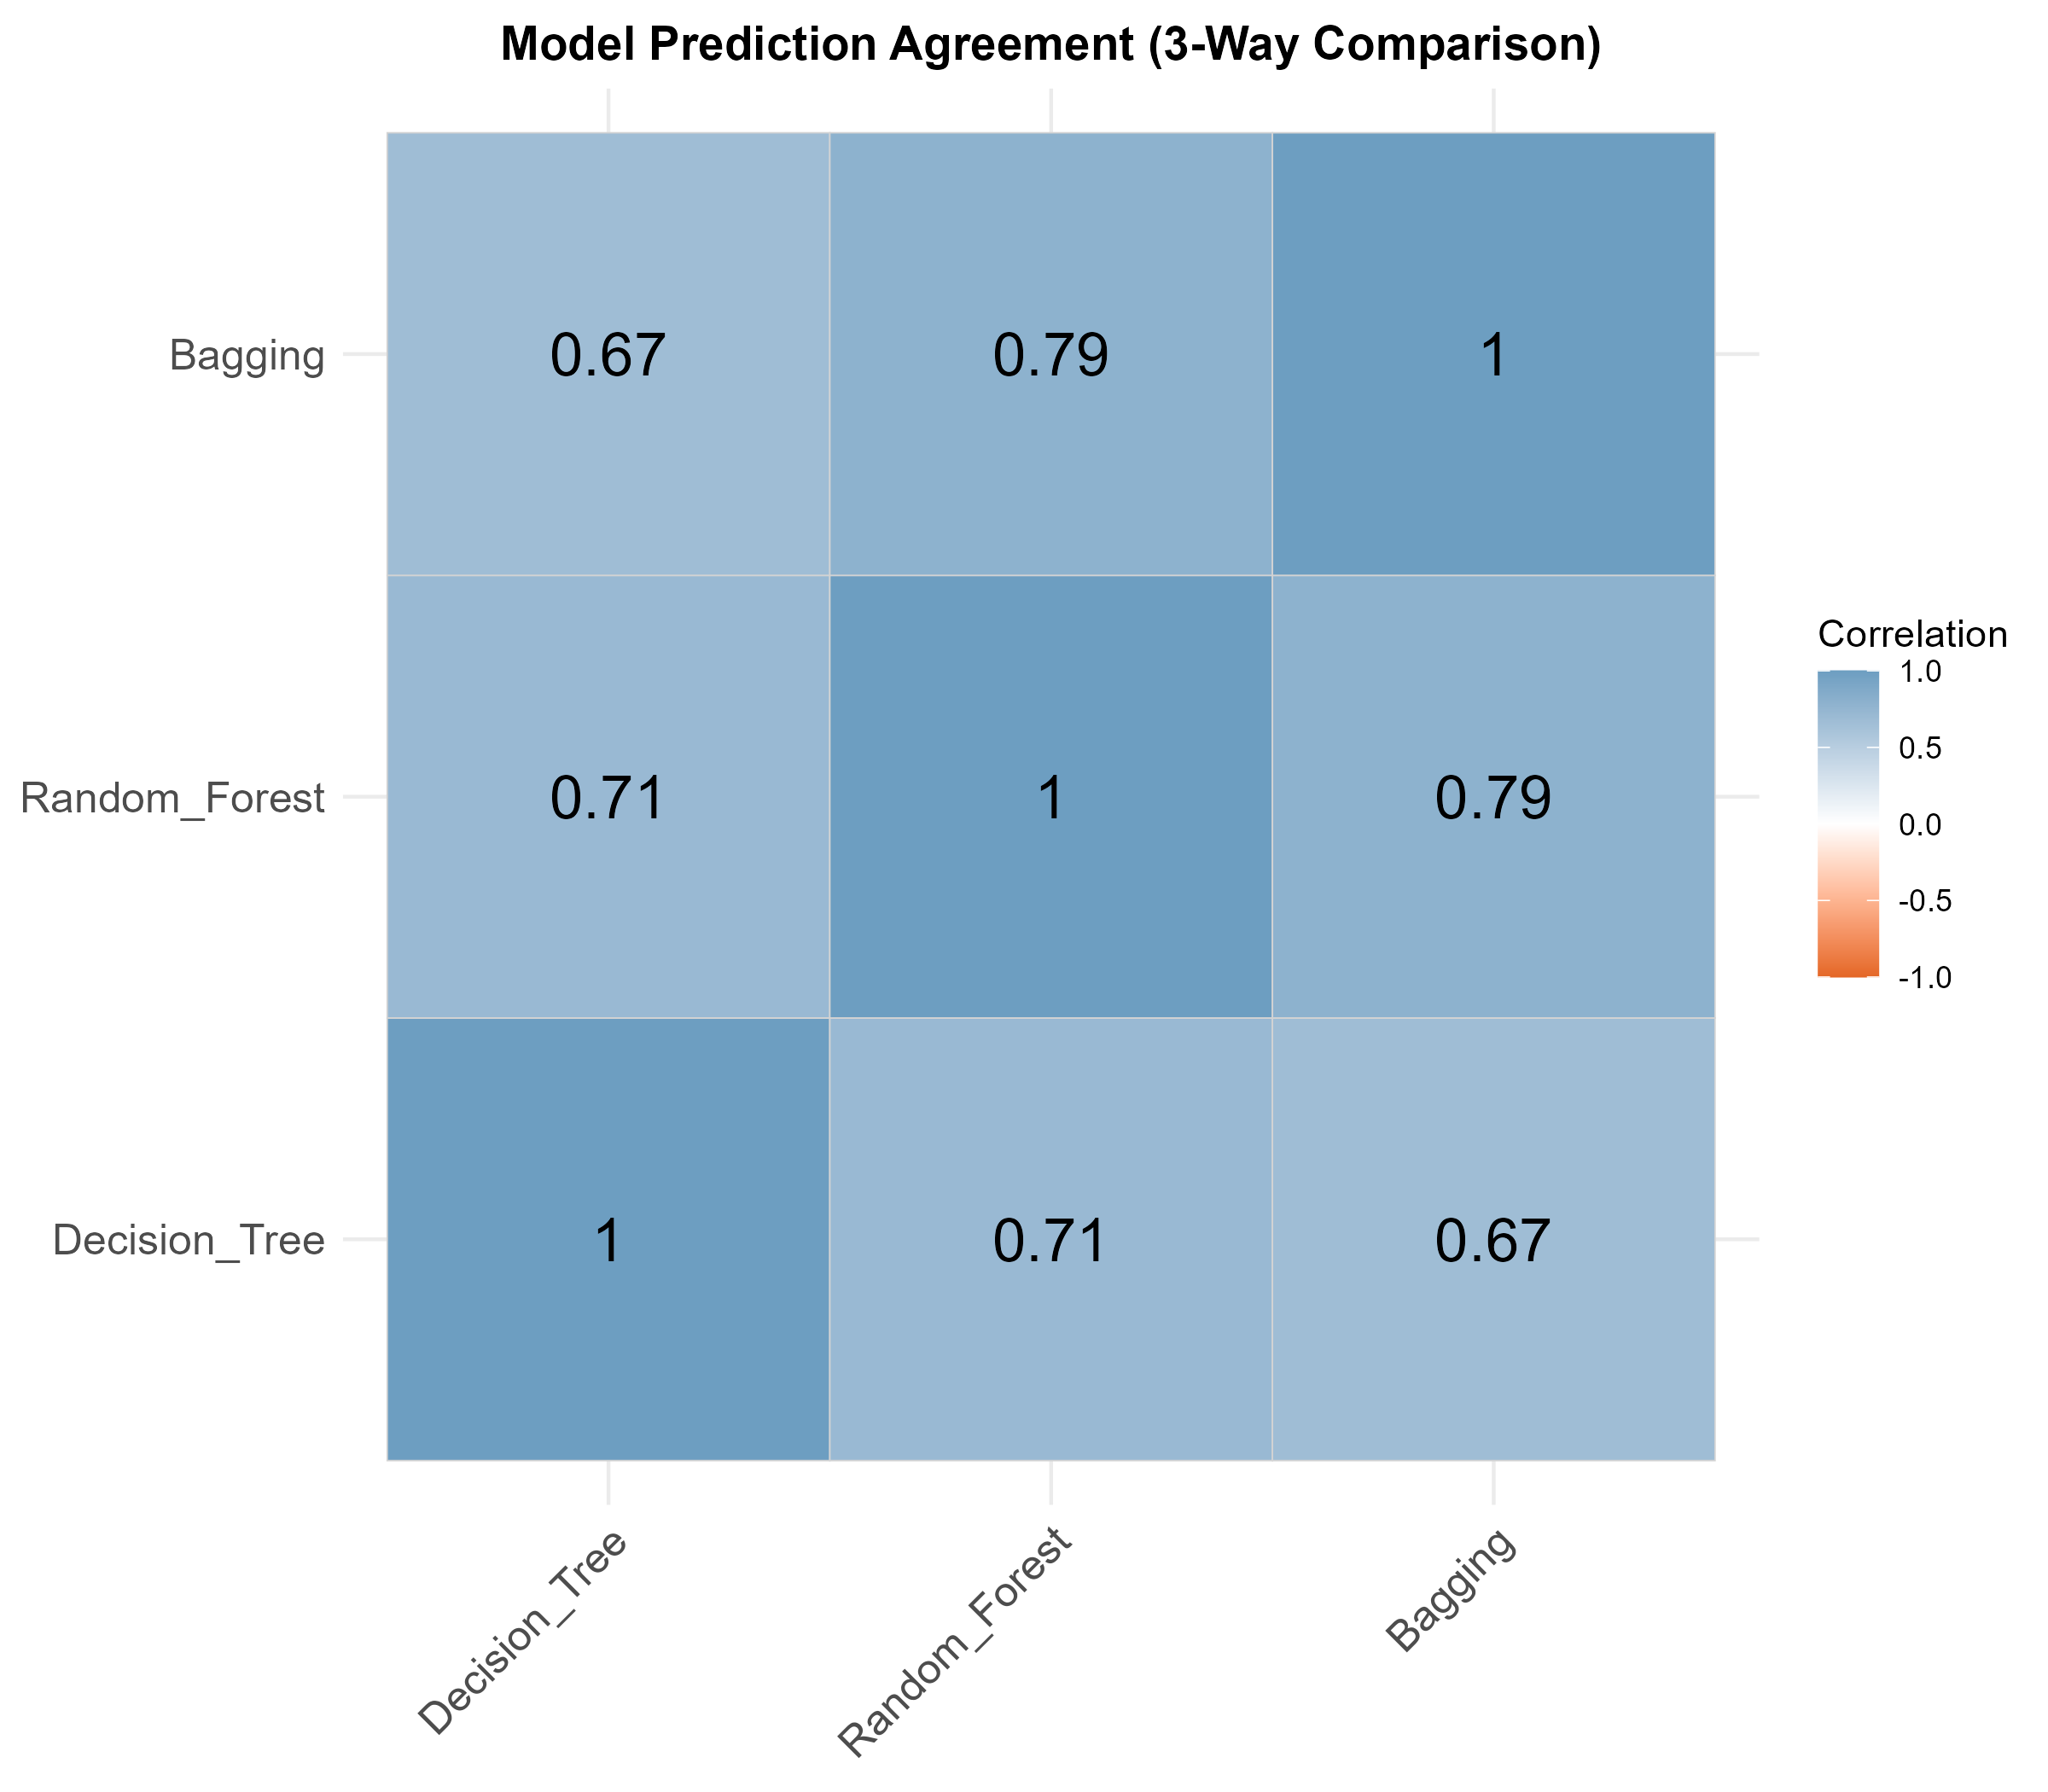
\includegraphics[scale=0.45]{model_agreement_correlation.png}}
	\caption{Model Agreement}
	\label{Tc_model_agreement}
\end{figure}

The correlation matrix in Figure \ref{Tc_model_agreement} confirms a strong positive alignment across all three models, with \textbf{Random Forest and Bagging} exhibiting the highest agreement ($r = 0.79$). This underscores their shared reliance on bootstrap aggregation, while the lack of perfect correlation highlights the successful decorrelation of learners through Random Forest's feature subsampling. 
 
Conversely, the \textbf{Decision Tree} shows the lowest agreement with \textbf{Bagging} ($r = 0.67$), reflecting the ensemble's ability to smooth the high variance and localized overfitting inherent in a single tree.\\
\indent The moderate correlation between the \textbf{Decision Tree and Random Forest} ($r = 0.71$) suggests that while the core logic remains consistent, the stochastic nature of the forest provides a distinct, more generalized predictive boundary. These results validate that the ensemble methods are successfully introducing the diversity required to improve model robustness over a standalone estimator.

\subsection{Comparative Model Performance}

\begin{figure}[htbp]
	\centerline{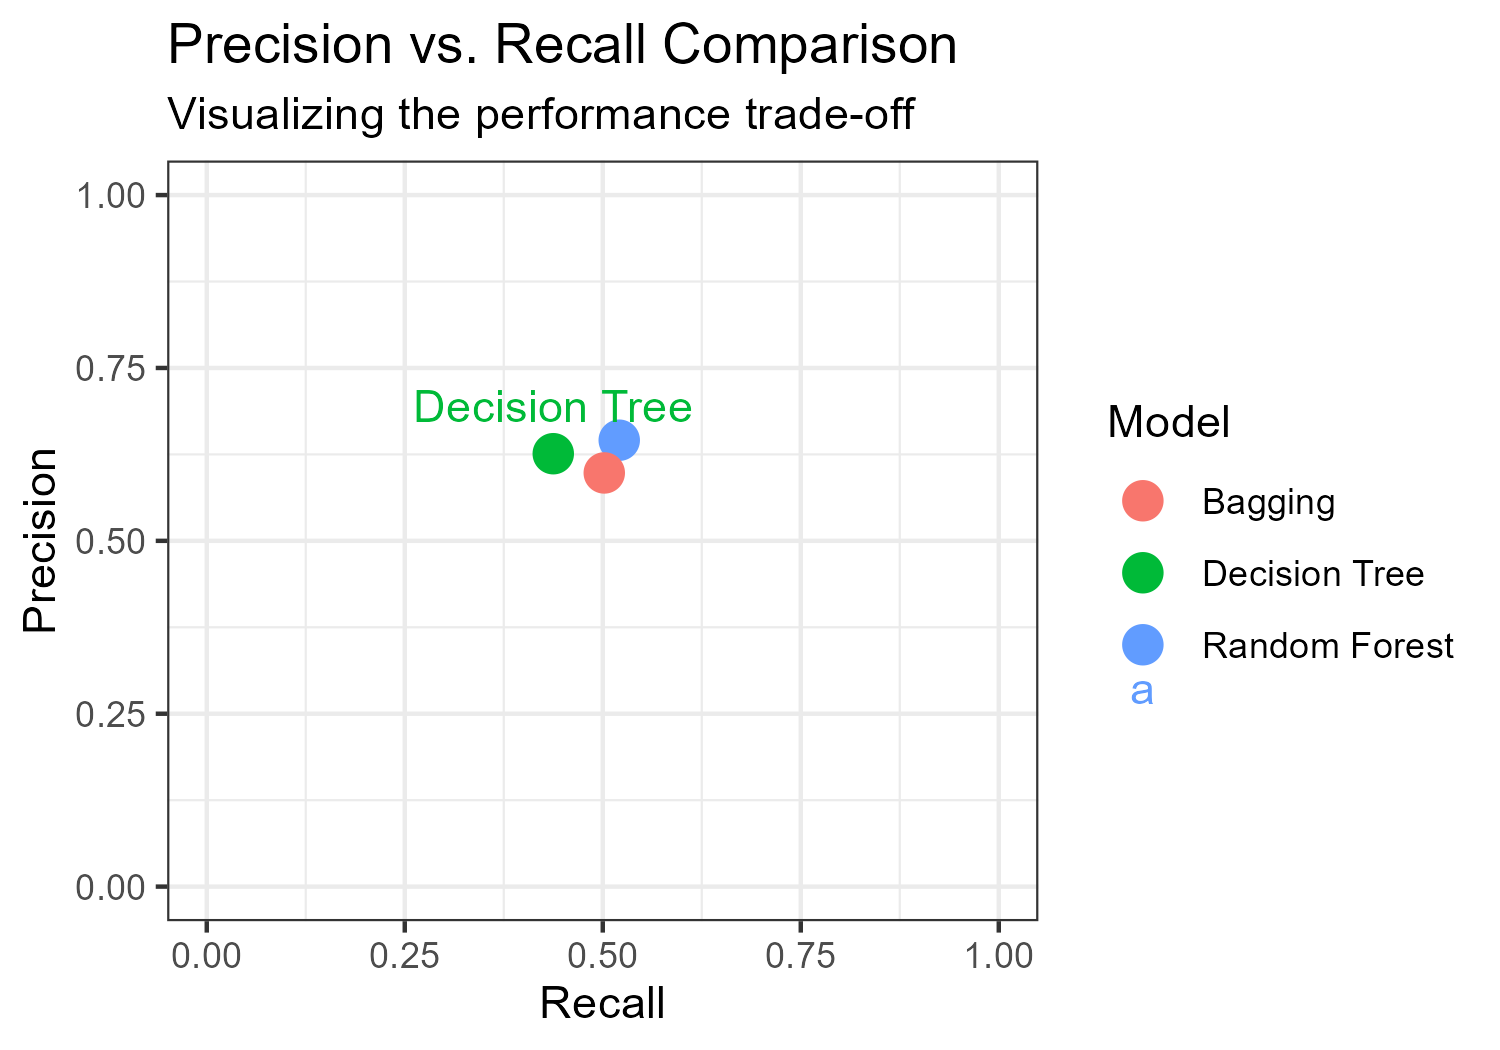
\includegraphics[scale=0.45]{precision_vs_Recall.png}}
	\caption{Precision-Recall Comparison Among Models}
	\label{Tc_precision_vs_Recall}
\end{figure}

The precision-recall visualization of Figure  \ref{Tc_precision_vs_Recall} indicates that the \textbf{Random Forest} model is the superior performer among the three candidates, achieving the highest balance with a precision of approximately $0.65$ and a recall of $0.52$. While the \textbf{Decision Tree} maintains a similar precision level to the Random Forest, it suffers from a notable deficit in recall ($\approx 0.43$), suggesting a higher rate of false negatives and a more restrictive classification boundary.\\
\indent Conversely, the \textbf{Bagging} model demonstrates an inverse trade-off; it matches the Random Forest's recall but exhibits the lowest precision ($\approx 0.60$) in the cohort.\\
\indent This suggests that while ensemble methods generally improved the model's ability to capture relevant instances compared to the base Decision Tree, the Random Forest's specific feature-subsampling approach was most effective at suppressing false positives without sacrificing sensitivity.

\section{\textbf{Conclusion(s)}}

This study demonstrates that while tree-based models are effective for financial classification, ensemble methods are essential for addressing the inherent class imbalance of telemarketing data. While the baseline \textbf{Decision Tree} achieved a high overall accuracy of 90.38\%, its low \textbf{Recall (43.75\%)} confirmed the anticipated majority-class bias, failing to identify more than half of the potential subscribers.\\
\indent In contrast, the \textbf{Random Forest} configuration proved to be the most robust predictive framework. By optimizing the feature space to achieve the highest \textbf{F1-Score (0.5765)} and \textbf{Recall (52.08\%)}, it stands as the superior model for improving bank subscription classification of this analysis.\\
\indent  Ultimately, the transition from a single-tree model to ensemble models like \textbf{Bagging} and \textbf{Random Forest} provided the stability necessary to capture nuanced subscriber signatures. By reducing variance and mitigating noise from the majority ``No'' class, these models offer a more reliable tool for targeting high-propensity clients.\\
\indent Future iterations of this analysis could enhance minority-class detection by incorporating advanced sampling techniques or boosting algorithms to further refine predictive precision for the ``Yes'' class.

\section*{\textbf{Appendix}}
	
\section*{Appendix A: Supplementary Materials and Software Usage}
\subsection*{Source Code Repository \label{app:code}}
The source code, data, and detailed implementation scripts for this project are available on GitHub (URL: \url{https://github.com/gaguillen4384-dev/Data-Science/tree/main/DataMining_2/Tree_Methods_Analysis_Bank_Marketing}).

\subsection*{Software Usage Acknowledgment}
The text and documentation were edited and refined using Google Gemini.

\begin{thebibliography}{9} % '9' is for formatting the numbering (up to 9 items)
	
\bibitem{moro2014}
Moro et al. (2014). Decision Support Systems 62, 22--31. (A data-driven approach to predict the success of bank telemarketing)
	
\end{thebibliography}

\vspace{12pt}

\end{document}
